%\immediate\write18{makeindex \jobname.nlo -s nomencl.ist -o \jobname.nls}
\documentclass[a4paper, twoside]{article}
%\usepackage[left=30mm,right=30mm,top=30mm,bottom=30mm]{geometry}
\usepackage[utf8]{inputenc}
\usepackage[T1]{fontenc}
\usepackage{textcomp}
\usepackage[english]{babel}
\usepackage{amsmath, amssymb, amsfonts}
\usepackage{gensymb}
\usepackage{float}
\usepackage{csquotes, xpatch}
\usepackage{graphicx}
\graphicspath{{./figures/}}
\usepackage{enumitem}
\setlist[description]{leftmargin=\parindent, labelindent=\parindent}
\usepackage{subcaption} %  for subfigures environments 
\usepackage[font={small},figurename=Fig.,labelfont={color=black,bf}]{caption}
\usepackage[toc,page]{appendix}
\usepackage[dvipsnames]{xcolor}
\usepackage{pdfpages}

\newcommand\myshade{85}
\colorlet{mylinkcolor}{violet}
\colorlet{mycitecolor}{YellowOrange}
\colorlet{myurlcolor}{Aquamarine}
\usepackage[unicode]{hyperref}
\hypersetup{
  linkcolor  = mylinkcolor!\myshade!black,
  citecolor  = mycitecolor!\myshade!black,
  urlcolor   = myurlcolor!\myshade!black,
  colorlinks = true}
\usepackage{cleveref}

\usepackage{pgfplots}
\DeclareUnicodeCharacter{2212}{−}
\usepgfplotslibrary{groupplots,dateplot}
\usetikzlibrary{patterns,shapes.arrows}
\pgfplotsset{compat=newest}

% nebo "iso-numeric", "iso-authoryear", sortlocale=cs_CZ, sorting=none,
\usepackage[style=iso-numeric, sortlocale=cs_CZ, sorting=none]{biblatex}
\addbibresource{bibliography.bib}

\pdfsuppresswarningpagegroup=1

\usepackage[]{nomencl}
\nomlabelwidth=15mm 

\makenomenclature

\begin{document}
\begin{titlepage}
    \begin{center}
        \vspace*{1cm}
        
        \LARGE
        Czech Technical University in Prag\\[0.1cm]
       	Faculty of Mechanical engineering\\[0.4cm]
		\Large
        Department of instrumentation and control enfineering\\[0.25cm]
        \large
        Automation and industry informatics\\

		\vfill
            
        
\includegraphics[width=0.6\textwidth]{lion_white}
                    
        \vfill
        \Large
        Master Thesis

        \vspace{0.8cm}           

        \Huge
        \textbf{Title}
            
        \vspace{0.5cm}
        \LARGE
        Subtitle
        \vspace{3cm}

        \today \hfill \textbf{Roman Dušek}
    \end{center}
\end{titlepage}
\newpage
\tableofcontents
\newpage
\printnomenclature
\newpage
\nomenclature{NN}{Neural network}%
\nomenclature{RNN}{Recurrent Neural network}%
\nomenclature{GRU}{Gated Recurrent Unit}%
\nomenclature{LSTM}{Long-Short-Term Memory}%
\nomenclature{HONU}{High Order Neural Unit}%
\nomenclature{HONN}{High Order Neural Network}%
\nomenclature{RHONN}{Recurrent High Order Neural Network}%


\section{Introduction}
\label{sec:introduction}

\begin{figure}[H]
	\centering
	% This file was created by tikzplotlib v0.9.8.
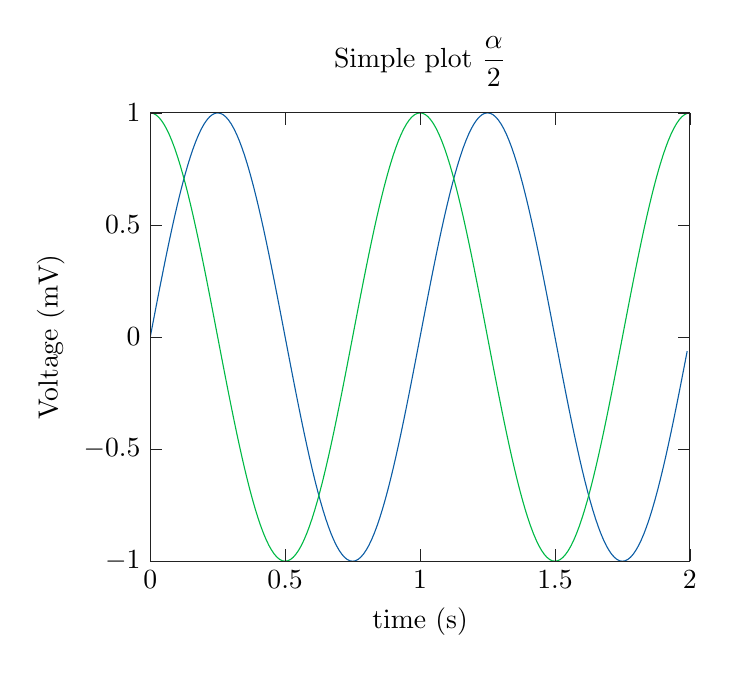
\begin{tikzpicture}

\definecolor{color0}{rgb}{0.0470588235294118,0.364705882352941,0.647058823529412}
\definecolor{color1}{rgb}{0,0.725490196078431,0.270588235294118}

\begin{axis}[
axis line style={white!13.3333333333333!black},
axis on top,
tick pos=both,
title={Simple plot \(\displaystyle \frac{\alpha}{2}\)},
x grid style={white!13.3333333333333!black},
xlabel={time (s)},
xmin=0, xmax=2,
xtick style={color=white!13.3333333333333!black},
y grid style={white!13.3333333333333!black},
ylabel={Voltage (mV)},
ymin=-1, ymax=1,
ytick style={color=white!13.3333333333333!black}
]
\addplot [color0]
table {%
0 0
0.01 0.0627905195293134
0.02 0.125333233564304
0.03 0.187381314585725
0.04 0.248689887164855
0.05 0.309016994374947
0.06 0.368124552684678
0.07 0.425779291565073
0.08 0.481753674101715
0.09 0.535826794978997
0.1 0.587785252292473
0.11 0.63742398974869
0.12 0.684547105928689
0.13 0.728968627421412
0.14 0.770513242775789
0.15 0.809016994374947
0.16 0.844327925502015
0.17 0.876306680043864
0.18 0.90482705246602
0.19 0.929776485888251
0.2 0.951056516295154
0.21 0.968583161128631
0.22 0.982287250728689
0.23 0.992114701314478
0.24 0.998026728428272
0.25 1
0.26 0.998026728428272
0.27 0.992114701314478
0.28 0.982287250728689
0.29 0.968583161128631
0.3 0.951056516295154
0.31 0.929776485888251
0.32 0.904827052466019
0.33 0.876306680043863
0.34 0.844327925502015
0.35 0.809016994374947
0.36 0.770513242775789
0.37 0.728968627421412
0.38 0.684547105928689
0.39 0.63742398974869
0.4 0.587785252292473
0.41 0.535826794978997
0.42 0.481753674101716
0.43 0.425779291565073
0.44 0.368124552684678
0.45 0.309016994374948
0.46 0.248689887164855
0.47 0.187381314585725
0.48 0.125333233564305
0.49 0.0627905195293136
0.5 1.22464679914735e-16
0.51 -0.0627905195293133
0.52 -0.125333233564304
0.53 -0.187381314585725
0.54 -0.248689887164855
0.55 -0.309016994374948
0.56 -0.368124552684678
0.57 -0.425779291565073
0.58 -0.481753674101715
0.59 -0.535826794978996
0.6 -0.587785252292473
0.61 -0.63742398974869
0.62 -0.684547105928689
0.63 -0.728968627421411
0.64 -0.770513242775789
0.65 -0.809016994374947
0.66 -0.844327925502015
0.67 -0.876306680043864
0.68 -0.90482705246602
0.69 -0.929776485888251
0.7 -0.951056516295154
0.71 -0.968583161128631
0.72 -0.982287250728689
0.73 -0.992114701314478
0.74 -0.998026728428272
0.75 -1
0.76 -0.998026728428272
0.77 -0.992114701314478
0.78 -0.982287250728689
0.79 -0.968583161128631
0.8 -0.951056516295154
0.81 -0.929776485888251
0.82 -0.90482705246602
0.83 -0.876306680043863
0.84 -0.844327925502016
0.85 -0.809016994374948
0.86 -0.77051324277579
0.87 -0.728968627421412
0.88 -0.684547105928689
0.89 -0.63742398974869
0.9 -0.587785252292473
0.91 -0.535826794978996
0.92 -0.481753674101715
0.93 -0.425779291565072
0.94 -0.368124552684678
0.95 -0.309016994374948
0.96 -0.248689887164855
0.97 -0.187381314585725
0.98 -0.125333233564305
0.99 -0.0627905195293133
1 -2.44929359829471e-16
1.01 0.0627905195293128
1.02 0.125333233564304
1.03 0.187381314585724
1.04 0.248689887164855
1.05 0.309016994374947
1.06 0.368124552684678
1.07 0.425779291565073
1.08 0.481753674101716
1.09 0.535826794978997
1.1 0.587785252292474
1.11 0.63742398974869
1.12 0.684547105928689
1.13 0.728968627421412
1.14 0.770513242775789
1.15 0.809016994374948
1.16 0.844327925502015
1.17 0.876306680043863
1.18 0.904827052466019
1.19 0.929776485888251
1.2 0.951056516295153
1.21 0.968583161128631
1.22 0.982287250728689
1.23 0.992114701314478
1.24 0.998026728428272
1.25 1
1.26 0.998026728428272
1.27 0.992114701314478
1.28 0.982287250728689
1.29 0.968583161128631
1.3 0.951056516295154
1.31 0.929776485888252
1.32 0.904827052466019
1.33 0.876306680043863
1.34 0.844327925502015
1.35 0.809016994374948
1.36 0.770513242775789
1.37 0.728968627421411
1.38 0.684547105928688
1.39 0.63742398974869
1.4 0.587785252292473
1.41 0.535826794978997
1.42 0.481753674101716
1.43 0.425779291565074
1.44 0.368124552684678
1.45 0.309016994374948
1.46 0.248689887164855
1.47 0.187381314585726
1.48 0.125333233564304
1.49 0.0627905195293134
1.5 3.67394039744206e-16
1.51 -0.0627905195293127
1.52 -0.125333233564303
1.53 -0.187381314585725
1.54 -0.248689887164855
1.55 -0.309016994374947
1.56 -0.368124552684677
1.57 -0.425779291565073
1.58 -0.481753674101716
1.59 -0.535826794978997
1.6 -0.587785252292473
1.61 -0.637423989748691
1.62 -0.684547105928689
1.63 -0.728968627421412
1.64 -0.770513242775789
1.65 -0.809016994374947
1.66 -0.844327925502016
1.67 -0.876306680043863
1.68 -0.904827052466019
1.69 -0.929776485888251
1.7 -0.951056516295153
1.71 -0.968583161128631
1.72 -0.982287250728688
1.73 -0.992114701314478
1.74 -0.998026728428272
1.75 -1
1.76 -0.998026728428272
1.77 -0.992114701314478
1.78 -0.982287250728689
1.79 -0.968583161128631
1.8 -0.951056516295154
1.81 -0.929776485888252
1.82 -0.904827052466019
1.83 -0.876306680043863
1.84 -0.844327925502015
1.85 -0.809016994374948
1.86 -0.770513242775789
1.87 -0.728968627421411
1.88 -0.684547105928689
1.89 -0.63742398974869
1.9 -0.587785252292473
1.91 -0.535826794978996
1.92 -0.481753674101716
1.93 -0.425779291565074
1.94 -0.368124552684678
1.95 -0.309016994374948
1.96 -0.248689887164856
1.97 -0.187381314585726
1.98 -0.125333233564304
1.99 -0.0627905195293135
};
\addplot [color1]
table {%
0 1
0.01 0.998026728428272
0.02 0.992114701314478
0.03 0.982287250728689
0.04 0.968583161128631
0.05 0.951056516295154
0.06 0.929776485888251
0.07 0.904827052466019
0.08 0.876306680043864
0.09 0.844327925502015
0.1 0.809016994374947
0.11 0.770513242775789
0.12 0.728968627421412
0.13 0.684547105928689
0.14 0.63742398974869
0.15 0.587785252292473
0.16 0.535826794978997
0.17 0.481753674101715
0.18 0.425779291565073
0.19 0.368124552684678
0.2 0.309016994374947
0.21 0.248689887164855
0.22 0.187381314585725
0.23 0.125333233564304
0.24 0.0627905195293135
0.25 6.12323399573677e-17
0.26 -0.0627905195293134
0.27 -0.125333233564304
0.28 -0.187381314585725
0.29 -0.248689887164855
0.3 -0.309016994374947
0.31 -0.368124552684678
0.32 -0.425779291565073
0.33 -0.481753674101715
0.34 -0.535826794978997
0.35 -0.587785252292473
0.36 -0.63742398974869
0.37 -0.684547105928689
0.38 -0.728968627421411
0.39 -0.770513242775789
0.4 -0.809016994374947
0.41 -0.844327925502015
0.42 -0.876306680043863
0.43 -0.904827052466019
0.44 -0.929776485888251
0.45 -0.951056516295154
0.46 -0.968583161128631
0.47 -0.982287250728689
0.48 -0.992114701314478
0.49 -0.998026728428272
0.5 -1
0.51 -0.998026728428272
0.52 -0.992114701314478
0.53 -0.982287250728689
0.54 -0.968583161128631
0.55 -0.951056516295153
0.56 -0.929776485888251
0.57 -0.904827052466019
0.58 -0.876306680043864
0.59 -0.844327925502015
0.6 -0.809016994374947
0.61 -0.770513242775789
0.62 -0.728968627421412
0.63 -0.684547105928689
0.64 -0.63742398974869
0.65 -0.587785252292473
0.66 -0.535826794978996
0.67 -0.481753674101715
0.68 -0.425779291565072
0.69 -0.368124552684678
0.7 -0.309016994374948
0.71 -0.248689887164855
0.72 -0.187381314585725
0.73 -0.125333233564305
0.74 -0.0627905195293132
0.75 -1.83697019872103e-16
0.76 0.0627905195293128
0.77 0.125333233564304
0.78 0.187381314585724
0.79 0.248689887164855
0.8 0.309016994374947
0.81 0.368124552684678
0.82 0.425779291565073
0.83 0.481753674101716
0.84 0.535826794978996
0.85 0.587785252292473
0.86 0.637423989748689
0.87 0.684547105928689
0.88 0.728968627421411
0.89 0.770513242775789
0.9 0.809016994374947
0.91 0.844327925502015
0.92 0.876306680043864
0.93 0.90482705246602
0.94 0.929776485888251
0.95 0.951056516295154
0.96 0.968583161128631
0.97 0.982287250728689
0.98 0.992114701314478
0.99 0.998026728428272
1 1
1.01 0.998026728428272
1.02 0.992114701314478
1.03 0.982287250728689
1.04 0.968583161128631
1.05 0.951056516295154
1.06 0.929776485888251
1.07 0.90482705246602
1.08 0.876306680043863
1.09 0.844327925502015
1.1 0.809016994374947
1.11 0.770513242775789
1.12 0.728968627421411
1.13 0.684547105928688
1.14 0.63742398974869
1.15 0.587785252292473
1.16 0.535826794978997
1.17 0.481753674101716
1.18 0.425779291565073
1.19 0.368124552684679
1.2 0.309016994374948
1.21 0.248689887164855
1.22 0.187381314585725
1.23 0.125333233564305
1.24 0.0627905195293133
1.25 3.06161699786838e-16
1.26 -0.0627905195293127
1.27 -0.125333233564304
1.28 -0.187381314585725
1.29 -0.248689887164855
1.3 -0.309016994374947
1.31 -0.368124552684677
1.32 -0.425779291565073
1.33 -0.481753674101716
1.34 -0.535826794978997
1.35 -0.587785252292473
1.36 -0.637423989748691
1.37 -0.684547105928689
1.38 -0.728968627421412
1.39 -0.770513242775789
1.4 -0.809016994374947
1.41 -0.844327925502015
1.42 -0.876306680043863
1.43 -0.904827052466019
1.44 -0.929776485888251
1.45 -0.951056516295153
1.46 -0.968583161128631
1.47 -0.982287250728688
1.48 -0.992114701314478
1.49 -0.998026728428272
1.5 -1
1.51 -0.998026728428272
1.52 -0.992114701314478
1.53 -0.982287250728689
1.54 -0.968583161128631
1.55 -0.951056516295154
1.56 -0.929776485888252
1.57 -0.904827052466019
1.58 -0.876306680043863
1.59 -0.844327925502015
1.6 -0.809016994374948
1.61 -0.770513242775789
1.62 -0.728968627421411
1.63 -0.684547105928689
1.64 -0.63742398974869
1.65 -0.587785252292473
1.66 -0.535826794978996
1.67 -0.481753674101716
1.68 -0.425779291565074
1.69 -0.368124552684678
1.7 -0.309016994374948
1.71 -0.248689887164856
1.72 -0.187381314585726
1.73 -0.125333233564304
1.74 -0.0627905195293134
1.75 -4.28626379701574e-16
1.76 0.0627905195293126
1.77 0.125333233564303
1.78 0.187381314585725
1.79 0.248689887164855
1.8 0.309016994374947
1.81 0.368124552684677
1.82 0.425779291565073
1.83 0.481753674101715
1.84 0.535826794978997
1.85 0.587785252292473
1.86 0.63742398974869
1.87 0.684547105928689
1.88 0.728968627421412
1.89 0.770513242775789
1.9 0.809016994374947
1.91 0.844327925502016
1.92 0.876306680043863
1.93 0.904827052466019
1.94 0.929776485888251
1.95 0.951056516295153
1.96 0.968583161128631
1.97 0.982287250728688
1.98 0.992114701314478
1.99 0.998026728428272
};
\end{axis}

\end{tikzpicture}

	\caption{Testing tikz2plot}
	\label{fig:}
\end{figure}

\section{Background}
\label{sec:background}

\subsection{Supervised learning}
\label{sub:supervised_learning}

\subsection{Neural networks}
\label{sub:neural_networks}

\subsubsection{Perceptron}
\label{ssub:perceptron}

\subsubsection{Learning and optimalization}
\label{ssub:learning_and_optimalization}

\subsection{Recurrent neural networks}
\label{sub:recurrent_neural_networks}


\subsubsection{Vanilla version}
\label{ssub:vanilla_version}

\subsubsection{Long-short-term-memories}
\label{ssub:long_short_term_memories}

\subsubsection{Gated recurrent units}
\label{ssub:gated_recurrent_units}


\subsubsection{Other types of RNN}
\label{ssub:other_types_of_rnn}

\subsubsection{Problems using RNN}
\label{ssub:problems_using_rnn}


\subsection{High order neural networks}
\label{sub:high_order_neural_networks}

\subsubsection{High order neural unit}
\label{ssub:high_order_neural_unit}

\subsubsection{Recurrent HONN}
\label{ssub:recurrent_honn}

\subsubsection{Problems using HONN}
\label{ssub:problems_using_honn}


\section{Experimental Setup}
\label{sec:experimental_setup}


\section{Discussion}
\label{sec:discussion}

\section{Conclusion}
\label{sec:conclusion}



\newpage
\nocite{*}
\printbibliography
%\addcontentsline{toc}{part}{References}
\newpage

\appendix
\part*{Appendix}
\addcontentsline{toc}{part}{Appendix}


\end{document}
